\section{Transmission System Design}


\begin{frame}{}
    \tableofcontents[currentsection]
\end{frame}

\begin{frame}{HVAC transmission system for an OWPP}

What we want to design?
\begin{figure}[H] %Recorda fixar la posició de les figures si no
  \centering
  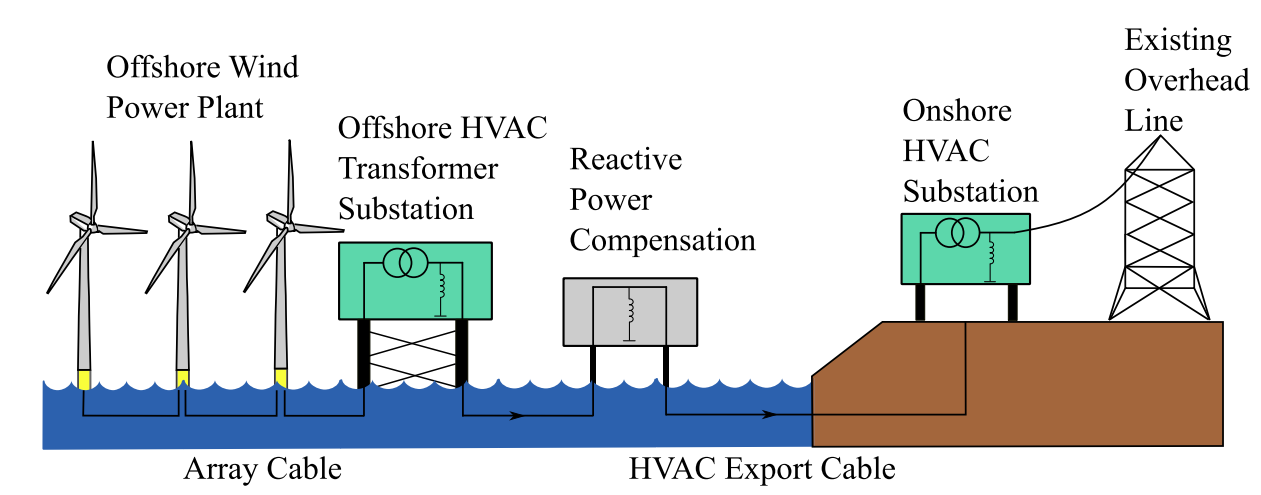
\includegraphics[width=0.75\textwidth]{imatges/layout.png}
  \caption{HVAC transmission system layout for an OWPP with reactive power compensation [\textit{check memory for citation}] .}
  \label{fig:fulltransmission} %Si es posen les etiquetes de forma ordenada, la vida es més fàcil...
\end{figure}

\end{frame}
\subsection{Reactive Power Compensation}

\begin{frame}{Reactive power compensation}
  
Underground HVAC cables have high capacitance, reactive power generation becomes a problem.
\begin{table}[h]
  \centering
  \begin{tabular}{c|c|c}
  \hline
   & Overhead Lines & Underground Lines \\
   \hline
  Capacitance Per Unit Length ($\mu$F/km) & 0.01 - 0.02  & 0.3 - 0.6 \\
  \hline
  \end{tabular}
  \caption{Comparison of Capacitance Per Unit Length of Overhead and Underground Lines.}
  \label{tab:capacitance_comparison}
  \end{table}

Reactive power compensation helps overcoming associated issues.

\begin{figure}
  \centering
  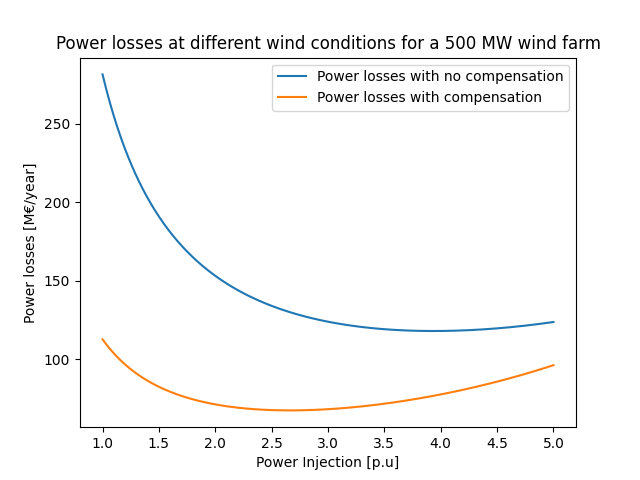
\includegraphics[width=0.400\textwidth]{imatges/why_compensation.png}
  \caption{Effect of including reactive power compensation.}
\end{figure}

\end{frame}

\begin{frame}{Shunt reactors}

Reactive power compensated by a shunt reactor is $Q_l = {Y}_{sh}\cdot U_{AC-N}^2$.
\begin{equation}
    {Y}_{sh} = \frac{1}{j\omega L}
\end{equation}
where $L$ is the inductance of the shunt reactor, $\omega$ the angular frequency and $U_{AC-N}^2$ the nominal transmission voltage.
\begin{figure}
  \centering
  
  \begin{minipage}{0.45\textwidth}
    \centering
    \scalebox{0.7}{
      \begin{circuitikz}
        \draw (0,0) to [generic, l=$\underline{y}_{sh}$] (0,-3) node[ground]{};
      \end{circuitikz}
    }
    \caption{Shunt reactor model.}
    \label{fig:shunt_reactor_model}
  \end{minipage}
  \begin{minipage}{0.45\textwidth}
    \centering
    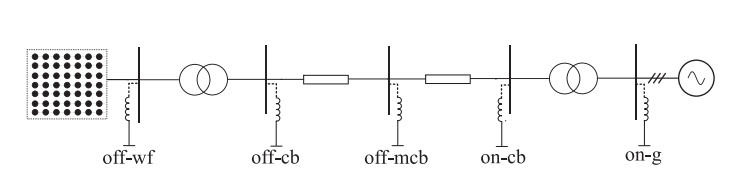
\includegraphics[width=\textwidth]{imatges/poss_position.png}
    \caption{Possible locations for the shunt reactors [\textit{check memory for citation}].}
    \label{fig:compensation_effect}
  \end{minipage}\hfill
\end{figure}

\end{frame}
\subsection{Elements Modelling}

\begin{frame}{Transmission system design}
  %Then the full transmission system looks like:

  \begin{figure}[h]
    \centering
    \resizebox{\textwidth}{!}{
    \begin{tikzpicture}[scale=1]
        \draw (0,0) rectangle (1.5,1.5);
        % Draw the dots
        \foreach \x in {0.3,0.6,0.9,1.2}
            \foreach \y in {0.3,0.6,0.9,1.2}
                \fill (\x,\y) circle (0.07);
        
        \draw (1.5,0.75) -- (3.5,0.75);
        \node at (3,0.75) [circle, draw=black, fill=black, inner sep=1pt, thick, label=above:$\textbf{1}$]{};
        \draw (3.5,0.75) to [generic, l=$\underline{Z}_{tr}$] (5,0.75);
        \draw (3,0.75) to [generic, l=$\underline{Y}_{tr}$] (3,-2) node[ground]{};
        \draw (3,0.4) -- (2,0.4);
        \draw (2,0.4) to [generic, l_=$\underline{Y}_{sh1}$] (2,-2)node[ground]{};
        \draw (5,0.75) -- (6,0.75);
        \node at (5.75,0.75) [circle, draw=black, fill=black, inner sep=1pt, thick, label=above:$\textbf{2}$]{};
        \draw (6,0.75) to [generic, l=$\underline{Z}_{\pi1}$] (7.5,0.75);
        \draw (5.75,0.75) to [generic, l=$\underline{Y}_{\pi1}$] (5.75,-2) node[ground]{};
        \draw (5.75,0.4) -- (5,0.4);
        \draw (5,0.4) to [generic, l_=$\underline{Y}_{sh2}$] (5,-2)node[ground]{};
        \draw (7.5,0.75) -- (10,0.75);
        \node at (9,0.75) [circle, draw=black, fill=black, inner sep=1pt, thick, label=above:$\textbf{3}$]{};
        \draw (8,0.75) to [generic, l_=$\underline{Y}_{\pi1}$] (8,-2) node[ground]{};
        \draw (9,0.75) to [generic, l^=$\underline{Y}_{sh3}$] (9,-2) node[ground]{};
        \draw (10,0.75) to [generic, l=$\underline{Y}_{\pi2}$] (10,-2)node[ground]{};
        \draw (10,0.75) to [generic, l=$\underline{Z}_{\pi2}$] (12.5,0.75);
        \draw (12.5,0.75) to [generic, l=$\underline{Y}_{\pi2}$] (12.5,-2) node[ground]{};
        \draw (12.5,0.4) -- (11.5,0.4);
        \node at (12.5,0.75) [circle, draw=black, fill=black, inner sep=1pt, thick, label=above:$\textbf{4}$]{};
        \draw (11.5,0.4) to [generic, l=$\underline{Y}_{sh4}$] (11.5,-2)node[ground]{};
        \draw (12.5,0.75) to [generic, l=$\underline{Z}_{tr}$] (15,0.75);
        \draw (15,0.75) to [generic, l=$\underline{Y}_{tr}$] (15,-2) node[ground]{};
        \node at (15,0.75) [circle, draw=black, fill=black, inner sep=1pt, thick, label=above:$\textbf{5}$]{};
        \draw (15,0.4) -- (14,0.4);
        \draw (14,0.4) to [generic, l=$\underline{Y}_{sh5}$] (14,-2) node[ground]{};
        \draw (15,0.75) to [generic, l=$\underline{Z}_{g}$](17,0.75);
        \draw (17,0.75) to[sV, l=$\underline{U}_{g}$] (17,-2) to (17,-2) node[ground]{};
        \node at (17,0.75) [circle, draw=black, fill=black, inner sep=1pt, thick, label=above:$\textbf{6}$]{};
    

    \end{tikzpicture}
    }
    \caption{Transmission system model and buses.}
    \label{fig:fullgrid}
    \end{figure}

    \begin{figure}[h]
      \begin{minipage}{0.45\textwidth}
        \centering
        \caption{Bus types.}
        \scalebox{0.7}{% Adjust the scale as needed
          \begin{tabular}{c|c}
            \hline
            \textbf{Bus Number} & \textbf{Bus Type} \\
            \hline
            1 & PQ \\
            2 & PQ \\
            3 & PQ \\
            4 & PQ \\
            5 & PQ \\
            6 & Slack \\
            \hline
          \end{tabular}
        }
        \label{tab:bus_types}
      \end{minipage}
      \begin{minipage}{0.45\textwidth}
        \centering
        \caption{Elements in the transmission system.}
        \scalebox{0.7}{% Adjust the scale as needed
          \begin{tabular}{c}
            \hline
            \textbf{Elements}\\
            \hline
            XPLE Cables \\
            Transformers \\
            Shunt reactors \\
            Switchgears \\
            Main Grid (given) \\
            Substation (cost dependent on OWPP) \\
            
            \hline
          \end{tabular}
        }
      \end{minipage}
    \end{figure}

\end{frame}













